\documentclass{article}
\usepackage{geometry}[letter]
\usepackage{amsmath}
\usepackage{amssymb}
\usepackage{gensymb}
\usepackage{graphicx}

\title{Smart Lock Network}

\author{
  lockNET \\ \\
  Kenneth Ozdowy (kozdowy@umich.edu), Erik Liubakka (eliubakk@umich.edu) \\
  Cristian G\'{o}mez Peces (peces@umich.edu)
}
\date{}

\begin{document}

\maketitle

\section{Customer}
Our target market is people in communal living spaces such as houses or shared
apartments, and who are looking for greater control over the security of their
own rooms by using a central system with credentials to allow access through
doors as opposed to a simple key mechanism.

\section{Value}

The first benefit is the added security of the doors via two-factor
authentication. Each door can only be unlocked either via something on you (i.e.
NFC via a phone) or a part of you (i.e. fingerprint). This method
surpasses using a physical key because it can not be as easily duplicated or
lockpicked, and is also convenient as the odds of losing a key are much greater
than losing a smartphone or your fingerprints. The state of the door can also be
sent to the owner, so if they forgot to lock it they can just use their phone to
do so (or set up autolock functionality).

The second benefit is that there is more freedom in terms of access. Each door
can have both blacklists and whitelists to outright deny or accept people, and
if someone's on neither, they can request access remotely instead, much quicker
than waiting for them to come home. 

\section{Approach}

The top level design is of a central hub with a number of nodes connected. The
hub is what allows users to communicate with the locks via a web interface. We
only want the hub to store what is necessary, acting as a control station while
each of the locks do most of the security part, making it much harder for
someone to spoof access rights.

When a scan occurs, the Arduino will compare the ID with its internal whitelist
and blacklist. If it's on the whitelist, the door will unlock. If it's on the
blacklist, not only will the door not unlock, but a record of the attempted
access is saved. If the ID is on neither list, the Arduino will inform the hub,
which sends out a notification to the lock's owner requesting approval. Upon
answer, the lock will unlock if approved. The request will also be recorded. If
the scan is via fingerprint, then only the prints already saved are allowed, and
no requests will be made if access is denied.

A similar notification method will be used to make changes to the locks. In
order to allow equal ownership, if somebody wishes to change a common lock, they
submit a request for the change, and the others must approve it first before it
becomes implemented.

The following diagrams will showcase the control flow for the various operations
that the system will perform:

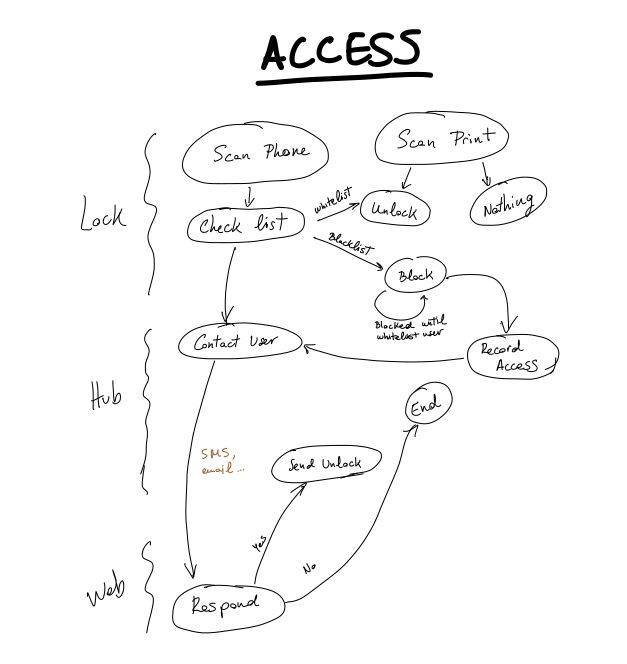
\includegraphics[scale=0.4]{access_graph.png}

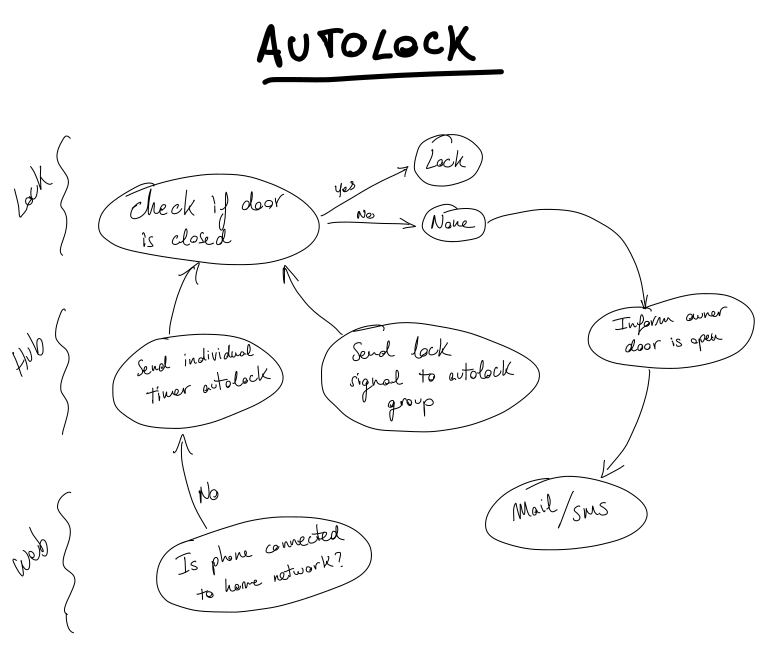
\includegraphics[scale=0.4]{autolock_graph.png}

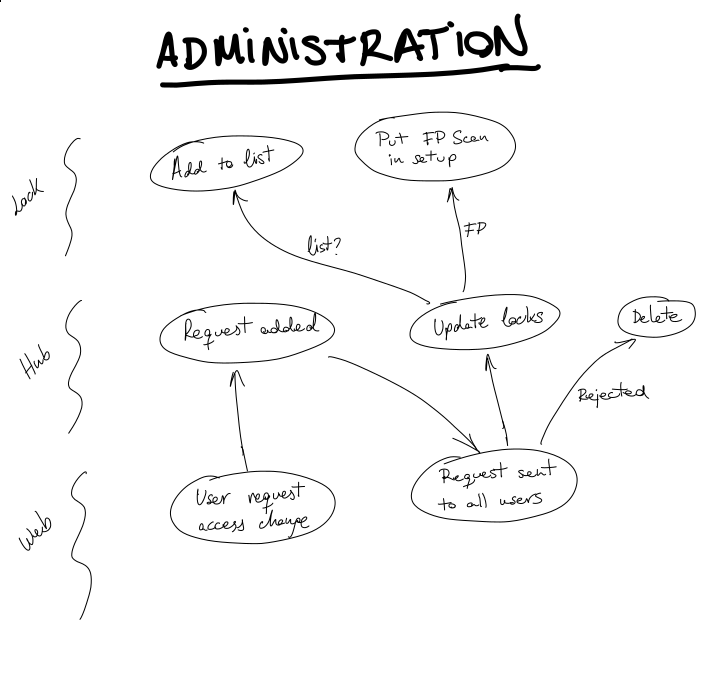
\includegraphics[scale=0.4]{admin_graph.png}

\section{Physical Components}


\subsection{Hub}

\noindent
Quantity: 1

\noindent
Base: \textbf{Intel Edison} (stock)

\noindent
Attachments:
\begin{itemize}

  \item LoRa transponder ($\thicksim$\$40)

  \item WiFi chip (already on board)

\end{itemize}

\subsection{Lock}

\noindent
Quantity: 2

\noindent
Base: \textbf{Arduino Uno} (stock)

\noindent
Attachments:
\begin{itemize}
  \item LoRa transponder ($\thicksim$\$40)
  \item $360\degree$ Servo motor ($\thicksim$\$14)
  \item Fingerprint scanner ($\thicksim$\$30)
  \item Physical lock ($\thicksim$\$10)
  \item NFC Scanner ($\thicksim$\$5)
  \item Magnetic contact switch ($\thicksim$\$4)
    %light sensor + LED? 
\end{itemize}

\section{Potential Components}
Instead of using regular Arduino Uno with the various sensors attached via IO
pins, we would design a custom Arduino board with the LoRa transponder and NFC
scanner as SMDs, and having dedicated pins for attaching the fingerprint scanner
and servo.
  

\end{document}
